\documentclass[a4paper,12pt]{report}
\usepackage[utf8]{inputenc}
\usepackage[francais]{babel}
\usepackage{fancyhdr}
\usepackage{graphicx}
\usepackage{tikz}
\usetikzlibrary{calc}
\usepackage{listings}
\usepackage{xcolor}
\definecolor{grey}{rgb}{0.9,0.9,0.9}
\usepackage{titlesec}
\usepackage{verbatim}
\usepackage{listings}
\usepackage{textcomp}
\usepackage{hyperref}
\usepackage{longtable}
\usepackage{colortbl}
\usepackage{amssymb}


\frenchbsetup{StandardLists=true}
\newcommand{\marge}{18mm}
\usepackage[left=\marge,right=\marge,top=\marge,bottom=\marge]{geometry}
\pagestyle{fancy}
\setlength{\headheight}{14pt}
\chead{
  \textbf{Binôme :} Douaille Erwan \& Yanis Nait Abdelaziz
  \hspace{2em}
  \textbf{Groupe :} M1 Info TI}
\renewcommand{\headrulewidth}{1pt}
\linespread{1}
\setlength{\columnseprule}{0.2pt}
\definecolor{javakeyword}{rgb}{0,0,0.5}
\definecolor{javastring}{rgb}{0,0.5,0}
\definecolor{javacomment}{rgb}{0.5,0.5,0.5}
\lstdefinestyle{java}{
   language=Java, basicstyle=\footnotesize,       % the size of the fonts that are used for the code
  numbers=left,                   % where to put the line-numbers
  numberstyle=\tiny\color{gray},  % the style that is used for the line-numbers
  stepnumber=1,                   % the step between two line-numbers. If it's 1, each line
                                  % will be numbered
  numbersep=5pt,                  % how far the line-numbers are from the code
  backgroundcolor=\color{white},  % choose the background color. You must add \usepackage{color}
  showspaces=false,               % show spaces adding particular underscores
  showstringspaces=false,         % underline spaces within strings
  showtabs=false,                 % show tabs within strings adding particular underscores
  frame=single,                   % adds a frame around the code
  rulecolor=\color{black},        % if not set, the frame-color may be changed on line-breaks within not-black text (e.g. commens (green here))
  tabsize=2,                      % sets default tabsize to 2 spaces
  captionpos=b,                   % sets the caption-position to bottom
  breaklines=true,                % sets automatic line breaking
  breakatwhitespace=false,        % sets if automatic breaks should only happen at whitespace
  title=\lstname,                 % show the filename of files included with \lstinputlisting;
   stringstyle=\color{javastring},
   keywordstyle=\color{javakeyword}\ttfamily\textbf,
   commentstyle=\color{javacomment}\ttfamily\textit
 }

\begin{document}



\makeatletter
\begin{titlepage}
\centering
\vspace{-10em}
{\LARGE \textbf{\textsc{Rapport de Projet RVI}}}\\
\vspace{3em}

\includegraphics[scale=0.6]{image/thalassa.png}\\
\vspace{3em}
{\LARGE \textsc{Projet Thalassa: simulation de plongée sous-marine}}\\

\vspace{8em}
Par\\
\vspace{1em}
{\LARGE \@author}\\

\vspace{2em}



\begin{tikzpicture}[remember picture,overlay]

\node [below left,xshift=-1cm, yshift=4cm] at (current page.south east){
\includegraphics[scale=0.6]{image/ustl1.png}};

\end{tikzpicture}
\end{titlepage}
\makeatother

\sloppy

\setcounter{page}{1} 
\newpage

\section*{Introduction}

Dans ce TP, nous allons comprendre comment obtenir des contours sur une image bruitée, ou non. Pour cela nous utiliserons le filtre Laplacien qui permet d'obtenir les contours ainsi que le LoG, une combinaison du filtre Laplacien et du filtre Gaussien.








\section*{Calcul du Laplacien}

Le Laplacien est un filtre qui correspond à la dérivée seconde d'une image. 
Il permet de mettre en évidence les contours des motifs de l'image. Nous allons appliquer ce filtre sur notre image spore.png et observer le résultat.


\begin{figure}[!ht]
	\center	
	
\includegraphics[scale=0.5]{image/laplacian_convolve1.png}	
	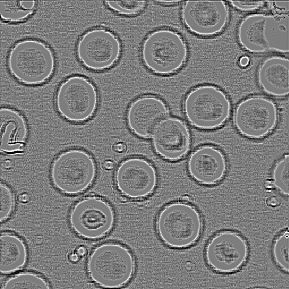
\includegraphics[scale=0.5]{image/laplacian_convolve2.png}	
	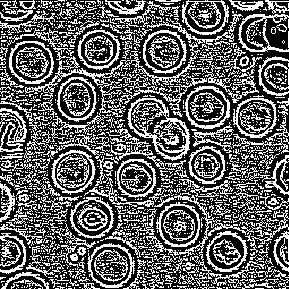
\includegraphics[scale=0.5]{image/laplacian_convolve4.png}	
\end{figure}


\begin{lstlisting}[style=Java]
FloatProcessor fpLaplacian = (FloatProcessor)(ip.duplicate().convertToFloat());
fpLaplacian.convolve(MASQUES_LAPLACIENS3x3[filtre], 3, 3);
this.imp = new ImagePlus("laplacian convolve", fpLaplacian);
this.imp.show();
\end{lstlisting}


Dans l'image de droite, qui est le résultat de spore.png sur laquelle on a appliqué notre filtre Laplacien,presque noire, on observe quelques contours. 
Pour observer plus distinctement cette image, nous avons modifié son contraste, pour obtenir l'image centrale. 
La dernière image correspond à l'application de Threshold (seuil).

Nous pouvons observer sur la dernière image que notre résultat du filtre Laplacien correspond bien au résultat attendu et est similaire à la dérivée seconde.
En effet on constate autour de nos motifs des contours noirs suivis d'un autre contour blanc. Ces "contours" sont la représentation des points de contour.

\begin{figure}[!ht]
	\center	
	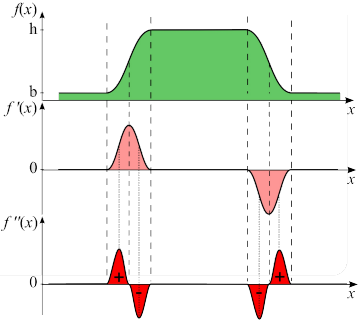
\includegraphics[scale=0.5]{image/laplacian_schema.png}
\end{figure}

Comme l'explique ce schéma lors d'une détection de contour, on fait un passage par zéro, + et ensuite -. 
Cette transition est symbolisée par le contour noir (+) et le blanc (-).

\begin{figure}[!ht]
	\center	
	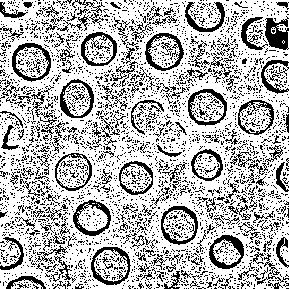
\includegraphics[scale=0.5]{image/laplacian_convolve5.png}
\end{figure}

En se rapprochant de la valeur 0 (içi -2.84 et 1.51) on observe que les contours obtenus ne sont pas uniformes et que la valeur de passage par zéro n'est pas toujours respectée.
Nous verrons dans la partie suivante que nous pouvons définir le seuil de passage à zéro.

\section*{Seuillage des passages par 0 du Laplacien}

Pour implémenter cet algorithme nous allons utiliser deux boucles pour parcourir l'image principale, incluant deux autres boucles permettant de parcours les voisins du pixel courrant.
Dans la boucle parcourant les voisins du pixel courrant, nous allons mémoriser la valeur min et le max parmis les voisins. Ensuite nous testerons le min et le max comme indiqué dans la formule.
Si min est inférieur à l'inverse du seuil et max supérieur au seuil, alors il s'agit d'un point contour et sa valeur sera 255 sinon 0.
Cette valeur est ensuite rangée dans la nouvelle image.

\begin{lstlisting}[style=Java]
ByteProcessor imZeros = new ByteProcessor(width,height);
		for (int i = 1; i < height-1; i++) {
			for (int j = 1; j < width-1; j++) {
				float min = imLaplacien.get(j,i);
				float max = imLaplacien.get(j,i);
				for (int x = -1; x < 2; x++) {
					for (int y = -1; y < 2; y++) {
						if (min>imLaplacien.get(x+j,y+i)) 
							min = imLaplacien.getf(x+j,y+i);						
						if (max<imLaplacien.get(x+j,y+i)) 
							max = imLaplacien.getf(x+j,y+i);
					}
				}
				if (min<-seuil && max>seuil) 
					imZeros.set(j, i, 255);
				else 
					imZeros.set(j, i, 0);	
			}
		}			
		return imZeros;
\end{lstlisting}

\newpage

\begin{figure}[!ht]
	\center	
	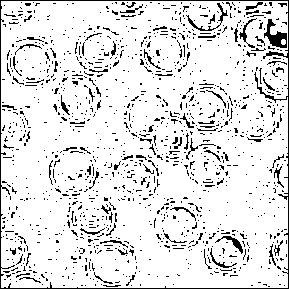
\includegraphics[scale=0.5]{image/laplacian_seuil0.png}
	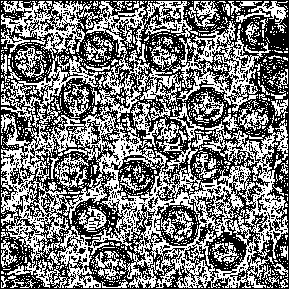
\includegraphics[scale=0.5]{image/laplacian_seuil3.png}
	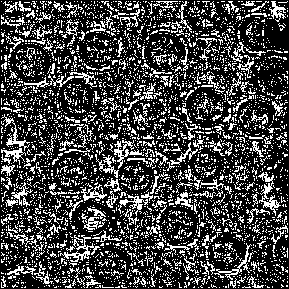
\includegraphics[scale=0.5]{image/laplacian_seuil6.png}
	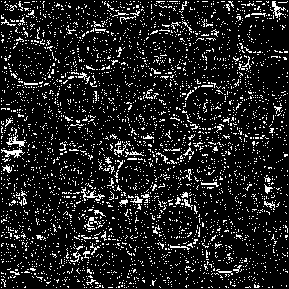
\includegraphics[scale=0.5]{image/laplacian_seuil10.png}
	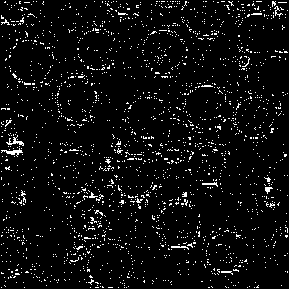
\includegraphics[scale=0.5]{image/laplacian_seuil15.png}
\end{figure}

Respectivement, les valeurs des seuils appliqués sont 0, 3, 6, 10 et 15. On observe que l'algorithme fonctionne parfaitement et que plus la valeur du seuil est élevée, plus les contours sont distincts. On observe également que l'image est énormément bruitée, ce qui limite la facilité de  distinguer correctement les contours.
En observant les images, la valeur de seuil 15 paraît içi parfaitement adaptée à nos besoins. Avec des valeurs plus élevées nous perdons de l'information malgrès un bruitage toujours présent.
La suite de ce TP propose d'utiliser des filtres pour supprimer le bruit. Un filtre de type Gaussien conviendrait parfaitement.

\newpage


\section*{Utilisation du filtre LoG et détection multi-échelles}

Notre masque doit obligatoirement être de taille impaire pour permettre d'avoir comme centre du masque la pixel courante.
tailleMasque et sigma sont liés car la taille du masque dépend de sigma. Sigma représente l'écart-type de la loi Gaussienne, donc plus cet écart-type est grand plus la taille du masque doit être grande, pour permettre de couvrir l'ensemble du bruit.


\begin{lstlisting}[style=Java]
int tailleMasque=(int)(7*sigma);
if(tailleMasque%2==0)
	tailleMasque++;
float[] masque=masqueLoG(tailleMasque,sigma);
if(sigma!=0) {
	Convolver conv = new Convolver();
	conv.setNormalize(false);
	conv.convolve(fpLaplacian,masque,tailleMasque,tailleMasque);
} else {
	fpLaplacian.convolve(MASQUES_LAPLACIENS3x3[filtre], 3, 3);
}
\end{lstlisting}

\begin{figure}[!ht]
	\center	
	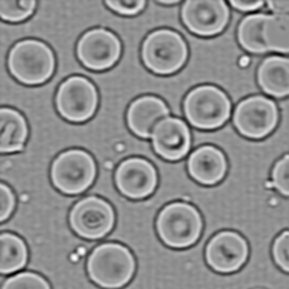
\includegraphics[scale=0.5]{image/laplacian_sigma2.png}
	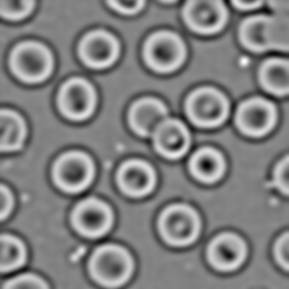
\includegraphics[scale=0.5]{image/laplacian_sigma4.png}
\end{figure}

L'application de LoG nous donne une image plus lisse et moin bruité. Plus sigma est important plus l'image est floue, comme visible dans les images, droite sigma vaut 2 et gauche sigma vaut 4.

\begin{figure}[!ht]
	\center	
	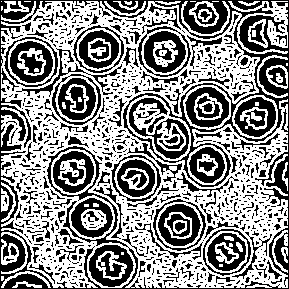
\includegraphics[scale=0.5]{image/laplacian_14.png}
	\caption{passage par 0 du LoG, sigma=1.4}
\end{figure}

\newpage
\begin{figure}[!ht]
	\center	
	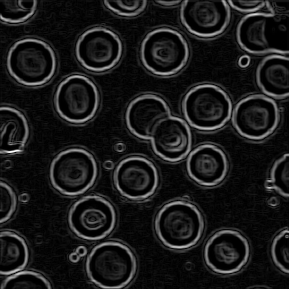
\includegraphics[scale=0.5]{image/gradient.png}
	\caption{Image de la norme du gradient de l'image Spores}
\end{figure}

\begin{figure}[!ht]
	\center	
	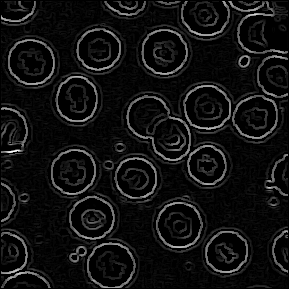
\includegraphics[scale=0.5]{image/q9.png}
	\caption{Question 9}
\end{figure}

\begin{figure}[!ht]
	\center	
	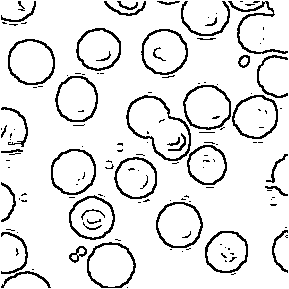
\includegraphics[scale=0.5]{image/q10.png}
	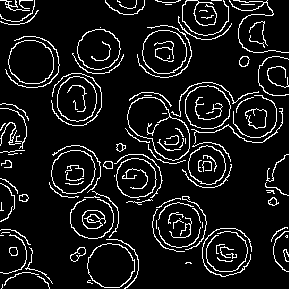
\includegraphics[scale=0.5]{image/q11.png}
\end{figure}

En comparant ces deux résultats on observe que celle obtenue par le plugin gradient (à droite), dessine les contours mais inclut plus d'éléments ce qui peut rendre complexe la détection des éléments.

Dans l'image obtenue à gauche on obtient uniquement des contours complètement formés et sans bruitage autour des contours. Nous appelons içi bruitage les éléments présents autour des contours de l'image de droite. Autrement dit, nos contours sont pleins.

\newpage

%%%%%%%%%%%%%%%%%%%%%%%%%%%%%%%%%%%%%%%%%% CONCLU
%%%%%%%%%%%%%%%%%%%%%%%%%%%%%%%%%%%%%%%%%%%%%%%%%
%%%%%%%%%%%%%%%%%%%%%%%%%%%%%%%%%%%%%%%%%%%%%%%%%
\section*{Conclusion}

Nous avons appris à obtenir des contours sur des images bruitées. Nous avons utilisé la techique de LoG qui nous permet d'obtenir les contours tout en ayant une image non bruitée. Cependant cette technique fait apparaître un flou sur l'image ce qui pourrait faire disparaître certains motifs et des contours de petite taille. Nous avons également remarqué que sur les dernières étapes une latence se faisait sentir lors du calcul des images.

\newpage

\section*{Listing}


\begin{lstlisting}[style=Java]
/**
 * My_Plugin_.java 
 * @  Douaille Erwan - Nait Abdelaziz Yanis
 *
 */

import ij.*;	// pour classes ImagePlus et IJ
import ij.gui.*;	// pour classes GenericDialog et DialogListener
import ij.plugin.filter.*;	// pour interface PlugInFilter et Convolver
import ij.process.*;	// pour classe ImageProcessor et sous-classes
import java.awt.*;		//pour classes AWTEvent, CheckBox, TextField
import java.util.Vector;	// pour classe Vector


public class My_Plugin implements PlugInFilter, DialogListener {
 
	private static int filtre=0;
	private final static String[] FILTRES_LAPLACIENS3x3 = {"Laplacien1", "Laplacien2", "Laplacien3","Laplacien4","Laplacien5"};
	private final static float[][] MASQUES_LAPLACIENS3x3 = {
		{0,1,0, 1,-4,1, 0,1,0},
		{1,0,1, 0,-4,0, 1,0,1},
		{1,1,1, 1,-8,1, 1,1,1},
		{1,2,1, 2,-12,2, 1,2,1},
		{1,4,1, 4,-20,4, 1,4,1}
	};
	private static float sigma=0.0f;
	private static boolean seuillageZeroCross=false;
	private static boolean seuilZeroCrossAuto=true;
	private static float seuilZeroCross=10f;
	
	private ImagePlus imp;

	public int setup(String arg, ImagePlus imp) {
		this.imp = imp;
		return PlugInFilter.DOES_8G;
	}

	public void run(ImageProcessor ip) {
		
		// Affichage de la fenetre de configuration
		if (!showDialog())
			return;

		// Titre et extension de l'image source
		String titre = imp.getTitle();
		String extension="";
		int index = titre.lastIndexOf('.');
		if (index>0)
			extension = titre.substring(index);
		else
			index = titre.length();
		titre = titre.substring(0,index);		
	
		FloatProcessor fpLaplacian = (FloatProcessor)(ip.duplicate().convertToFloat());

		//Q2 
		int tailleMasque=(int)(7*sigma);
		if(tailleMasque%2==0)
			tailleMasque++;
		float[] masque=masqueLoG(tailleMasque,sigma);


		if(sigma!=0) {
			Convolver conv = new Convolver();
			conv.setNormalize(false);
			conv.convolve(fpLaplacian,masque,tailleMasque,tailleMasque);
	 	} else {
			fpLaplacian.convolve(MASQUES_LAPLACIENS3x3[filtre], 3, 3);
		}

		this.imp = new ImagePlus("laplacian convolve", fpLaplacian);
		this.imp.show();
		
		if (seuillageZeroCross) {
			ImagePlus imsp = new ImagePlus("laplacian " + sigma, this.laplacienZero(fpLaplacian, seuilZeroCross));
			imsp.show();
		} 
	}
    
    public boolean showDialog() {
    	
		GenericDialog gd = new GenericDialog("Laplacian parameters");
		gd.addChoice("Laplacian filter type:", FILTRES_LAPLACIENS3x3, FILTRES_LAPLACIENS3x3[filtre]);
		gd.addNumericField("Gaussian filtering scale (0 for none)", sigma, 1);
		gd.addCheckbox("Threshold Laplacian zero-crossings", seuillageZeroCross);
		gd.addNumericField("Threshold value", seuilZeroCross, 0);
		gd.getComponent(gd.getComponentCount()-1).setEnabled(seuillageZeroCross && !seuilZeroCrossAuto); 
		gd.addCheckbox ("Auto threshold", seuilZeroCrossAuto);
		gd.getComponent(gd.getComponentCount()-1).setEnabled(seuillageZeroCross && seuilZeroCrossAuto); 
		gd.addDialogListener(this);     		// the DialogItemChanged method will be called on user input
		gd.showDialog();                		// display the dialog; preview runs in the background now
		if (gd.wasCanceled()) return false;

		filtre = gd.getNextChoiceIndex();
		sigma = (float) gd.getNextNumber();
		seuillageZeroCross = gd.getNextBoolean();
		seuilZeroCross = (float) gd.getNextNumber();
		seuilZeroCrossAuto = gd.getNextBoolean();

        return true;
    }	
    
	public boolean dialogItemChanged(GenericDialog gd, AWTEvent e) {
		
		Checkbox zcCheckbox = (Checkbox)gd.getCheckboxes().get(0);
		Checkbox zcAutoCheckbox = (Checkbox)gd.getCheckboxes().get(1);
		Vector numFields = gd.getNumericFields();
		TextField sigmaField = (TextField)numFields.get(1);
		TextField zcThresholdField = (TextField)numFields.get(1);
 		if (e!=null) {	
	        if (e.getSource() == zcCheckbox) { 
	        	zcThresholdField.setEnabled(zcCheckbox.getState()&&!zcAutoCheckbox.getState());
	        	zcAutoCheckbox.setEnabled(zcCheckbox.getState());
	        }
	        else if (e.getSource() == zcAutoCheckbox) {
	        	zcThresholdField.setEnabled(!zcAutoCheckbox.getState());
	        }
 		}
 		sigma = Float.valueOf(sigmaField.getText());
 		seuilZeroCross = Integer.valueOf(zcThresholdField.getText());
        return (!gd.invalidNumber() && sigma>=0 && seuilZeroCross>=0);
    }
	

	public ByteProcessor laplacienZero(ImageProcessor imLaplacien, Float seuil) {
		
		int width = imLaplacien.getWidth();
		int height = imLaplacien.getHeight();
		
		ByteProcessor imZeros = new ByteProcessor(width,height);
		for (int i = 1; i < height-1; i++) {
			for (int j = 1; j < width-1; j++) {
				float min = imLaplacien.get(j,i);
				float max = imLaplacien.get(j,i);
				for (int x = -1; x < 2; x++) {
					for (int y = -1; y < 2; y++) {
						if (min>imLaplacien.get(x+j,y+i)) {
							min = imLaplacien.getf(x+j,y+i);
						}
						if (max<imLaplacien.get(x+j,y+i)) {
							max = imLaplacien.getf(x+j,y+i);
						}
					}
				}
				if (min<-seuil && max>seuil) {
					imZeros.set(j, i, 255);
				} else {
					imZeros.set(j, i, 0);					
				}
			}
		}	
		
		return imZeros;
	}

    public static float[] masqueLoG(int tailleMasque, float sigma)
    {     
		short aperture = (short)(tailleMasque/2);
		double[][] LoG = new double[2*aperture+1][2*aperture+1];
		float[] out=new float[(2*aperture+1)*(2*aperture+1)];
		double sum=0, s2=Math.pow(sigma,2);
		int k=0;

		 // Calcul du masque LoG
		 for(int dy=-aperture;dy<=aperture;dy++)
		 {
			 for(int dx=-aperture;dx<=aperture;dx++)
			 {
				 double r2=-(dx*dx+dy*dy)/2.0/s2;
				 LoG[dy+aperture][dx+aperture]=-1/(Math.PI*s2*s2)*(1+r2)*Math.exp(r2);
				 sum+=LoG[dy+aperture][dx+aperture];
			 }
		 }
		 // Soustraction de la moyenne pour obtenir une somme nulle des coefs
		 sum=sum/(tailleMasque*tailleMasque);
		 for(int dy=-aperture;dy<=aperture;dy++)
			 for(int dx=-aperture;dx<=aperture;dx++)
				 out[k++]= (float)(LoG[dy+aperture][dx+aperture]-sum);
		 
		 return out;
    }
}
\end{lstlisting}

\end{document}